\documentclass[11pt]{article}
\usepackage[a4paper, left=0.75in, right=0.75in, top=0.5in, bottom=0.5in]{geometry}
\usepackage{amsmath, bm}
\usepackage{amssymb}
\usepackage{hyperref}
\hypersetup{
    colorlinks=true,
    linkcolor=blue,
    filecolor=magenta,      
    urlcolor=blue,
}
\usepackage{graphicx}
\graphicspath{ {.} }

\title{MSE 402 - Assignment 2}
\date{}
\author{Nishant Tatar - 21110223}

\begin{document}
\maketitle

\section{Question 1}
Molecular Dynamics refers to the evolution of state of a particular system. A system is initialised, and after that, the potentials and forces between all pairs of atoms/molecules is calculated from one time step to predict the next time step. However, Monte Carlo is a probabilistic technique, where each state has a certain probablity of existing, every 'time step' is a new configuration, from which the most probable states are calculated. \\
Where MD works on calculation and deterministic calculations, Monte Carlo works on probabilistic steps for generating each new configuration.\\ \\
Simple Monte Carlo would generate virtually infinite number of states, of which the majority would be discarded due to the probablity of them occuring being extremely low. The Implementation of the Metropolis algorithm in Monte Carlo ensures that computation is not wasted on generation of states which will not contribute to the final energy calculation. It biases the generation of new configurations towards states that contribute meaninfully to the integral. 
The Simple Monte Carlo method would generate all states with equal probability and then assign weights to each state with $\exp{\frac{-U_{r^N}}{k_{B}T}}$ whereas the Metropolis monte carlo method would generate states with the probability of $\exp{\frac{-U_{r^N}}{k_{B}T}}$ and then count each generated state equally.

\section{Question 2}
\subsection{SubQuestion A}
The "mol/swap" command in lammps performs Monte Carlo swaps of two specified atoms in a randomly selected molecule. This is useful when trying to acertain the miscibility of two different types of molecules. This process is faster than using molecular dynamics, because the swaps are done towards an energetically more favorable configuration.\\
It can also be used for Polymers, where swapping monomers inside the molecule can help find the energetically favorable fractions of the two molecules in the polymer.

\subsection{SubQuestion B}
Running the simulations for the various $\epsilon$ values, we find that for $\epsilon$ value of 0.1, the system is barely miscible and particles stay together amongst themselves. For $\epsilon$ of 1.0, the particles interact with one another as they would amongst themselves. For $\epsilon$ = 1.1, the system is extremely miscible, and the particles interact with each other more strongly than with their own types particles.\\
\textbf{For $\epsilon$ = 0.1} \\
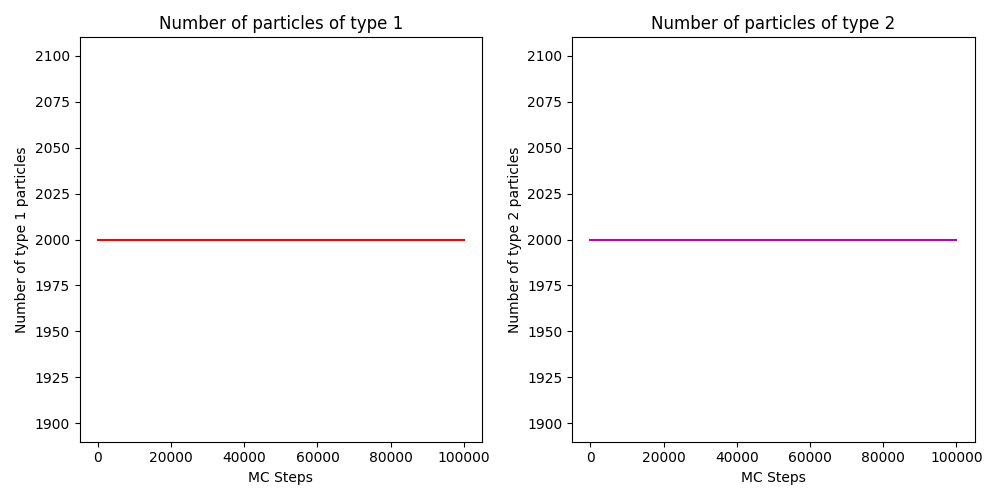
\includegraphics[scale=0.5]{Q2b_01ePlot.png} \\
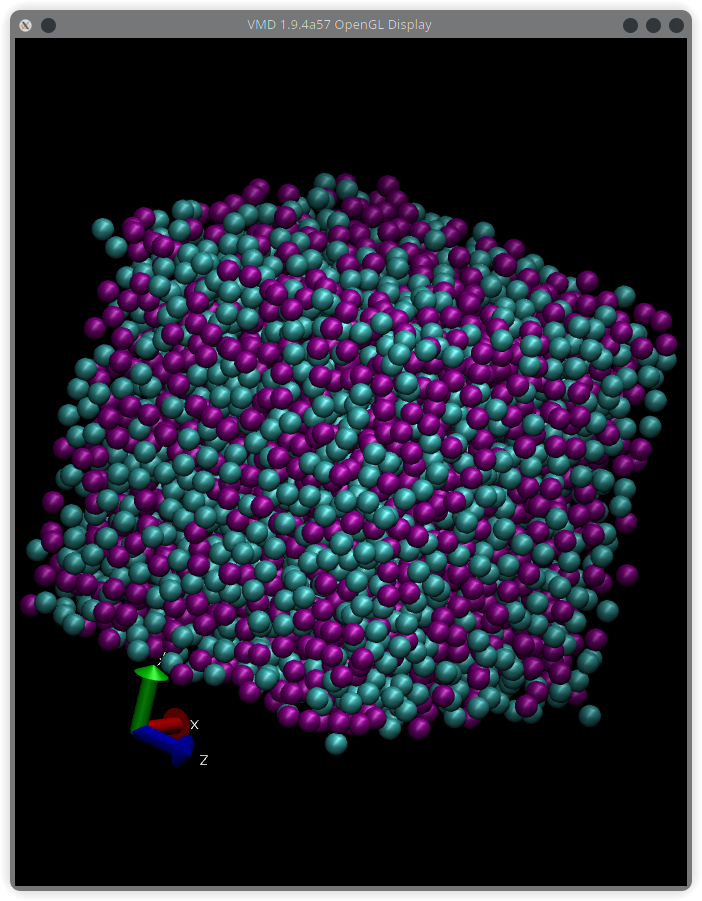
\includegraphics[scale=0.5]{Q2b_01eLF.png}\\
\textbf{For $\epsilon$ = 1.0} \\
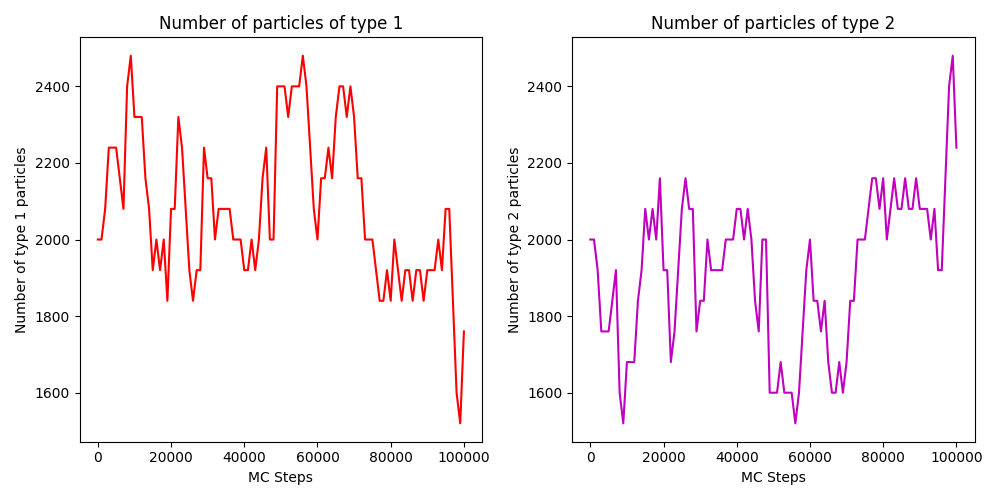
\includegraphics[scale=0.5]{Q2b_10ePlot.png} \\
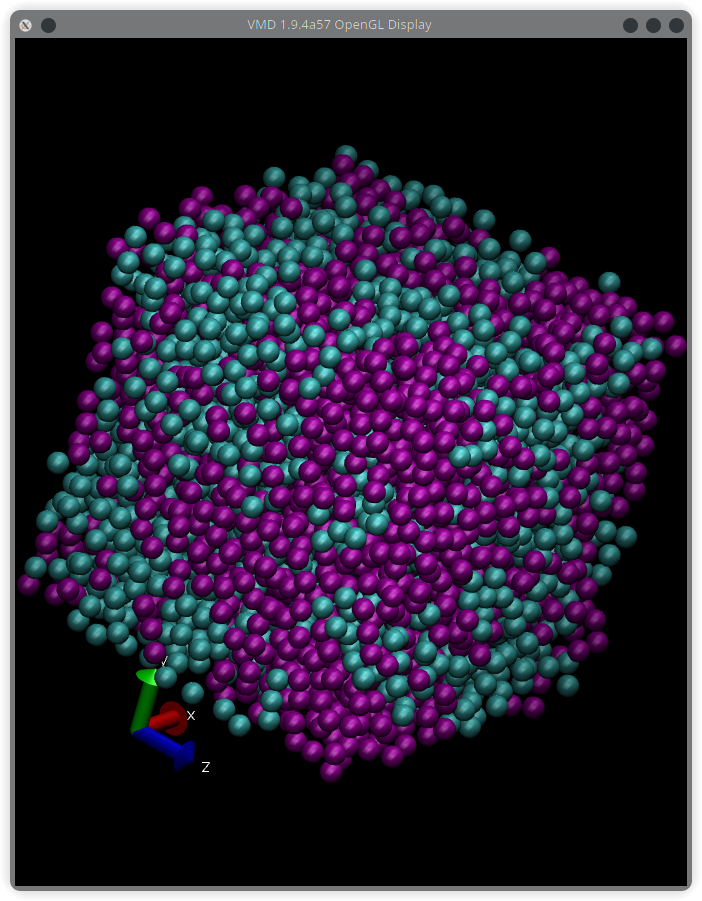
\includegraphics[scale=0.5]{Q2b_10eLF.png} \\
\textbf{For $\epsilon$ = 1.1} \\
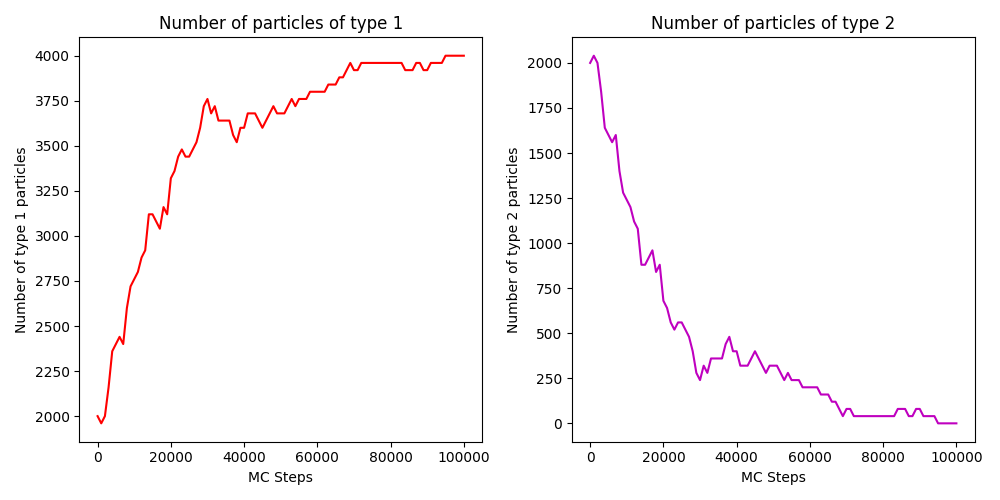
\includegraphics[scale=0.5]{Q2b_11ePlot.png} \\
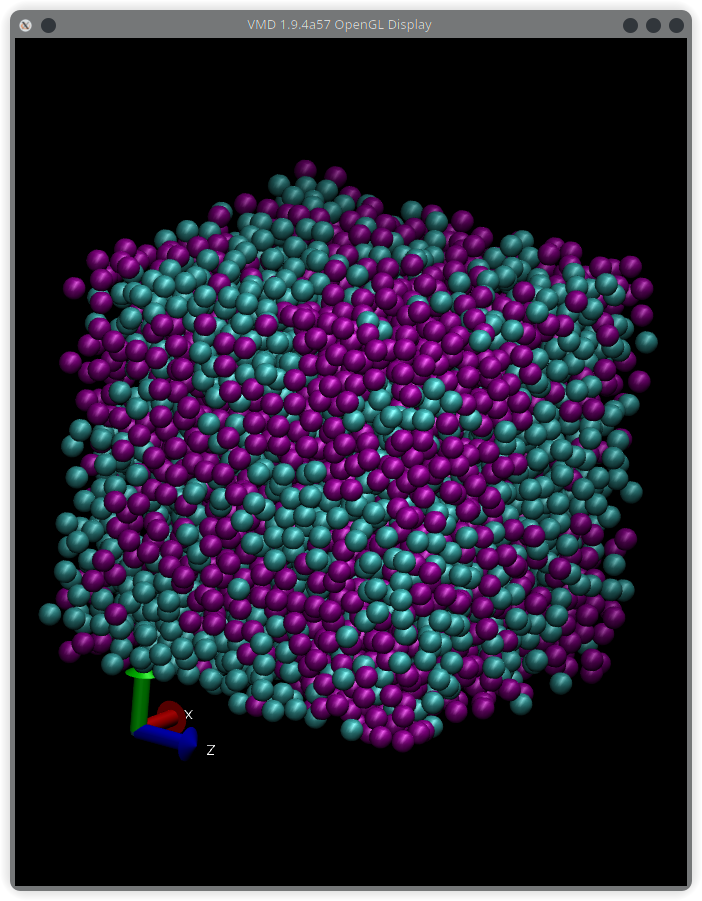
\includegraphics[scale=0.5]{Q2b_11eLF.png} \\

\section{Question 3}
\subsection{A}
Density Plot: \\
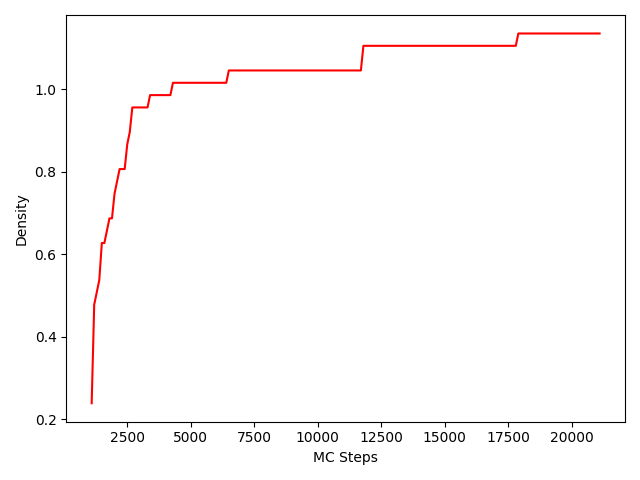
\includegraphics[scale=0.5]{Q3a_Density.png}\\
Variation of number of Oxygens and Hydrogens: \\
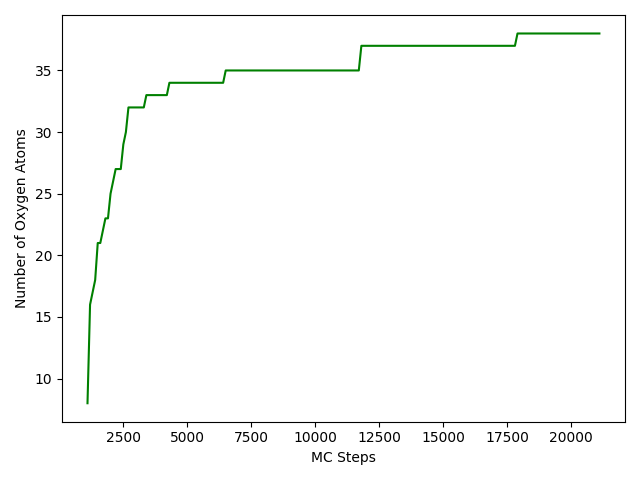
\includegraphics[scale=0.5]{Q3a_nO.png}
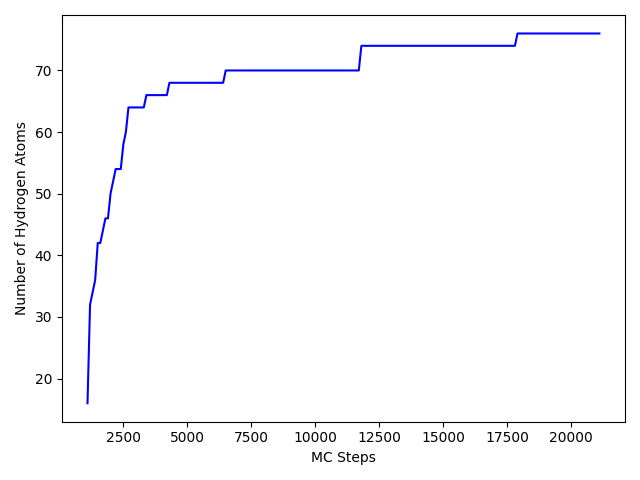
\includegraphics[scale=0.5]{Q3a_nH.png}\\
Visualisations for Initial and Final Frames: \\
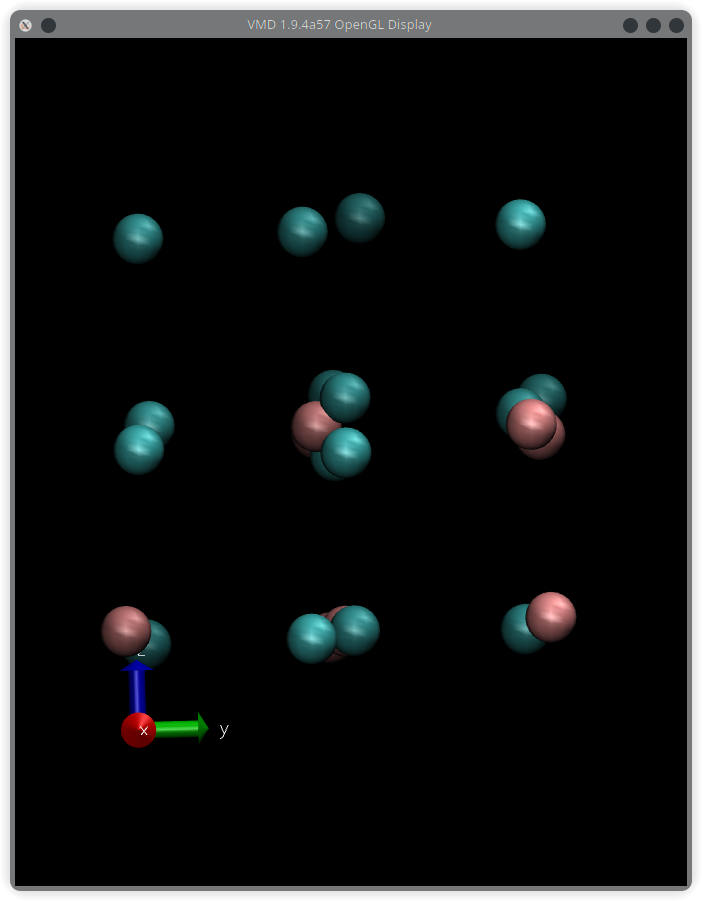
\includegraphics[scale=0.5]{Q3a_FF.png} 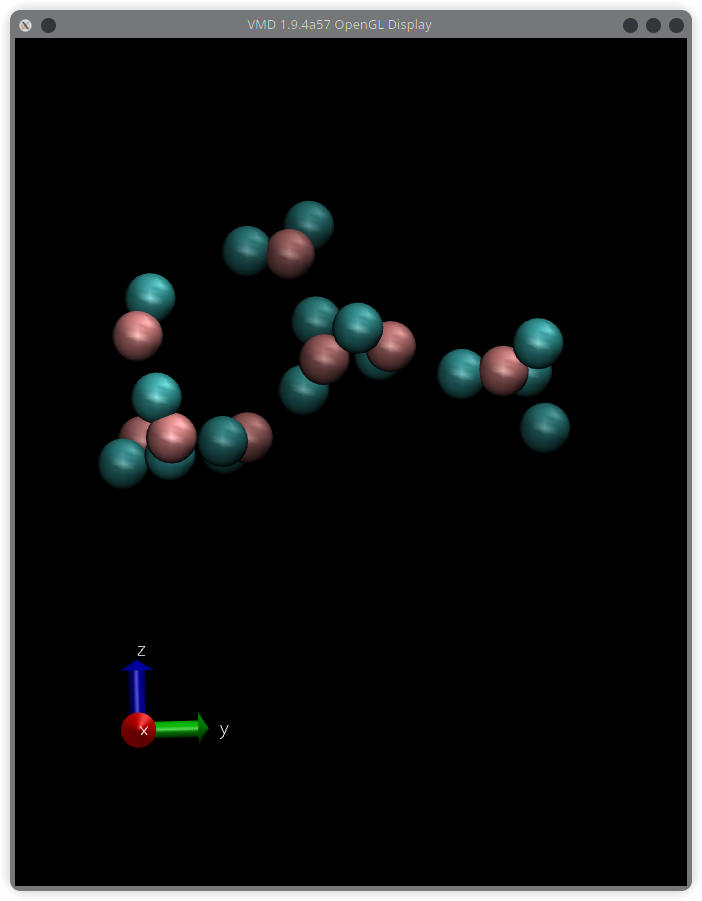
\includegraphics[scale=0.5]{Q3a_LF.png}
\subsection{B}
Visualisation before crack generation:\\
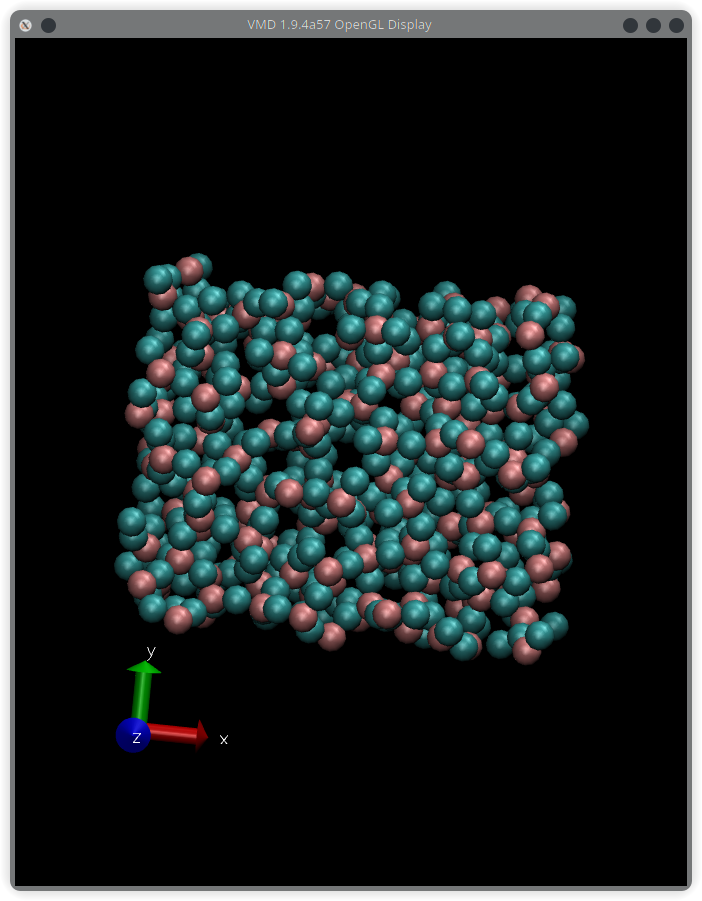
\includegraphics[scale=0.5]{Q3b_FF_Crack.png}\\
Visualisation after crack generation:\\
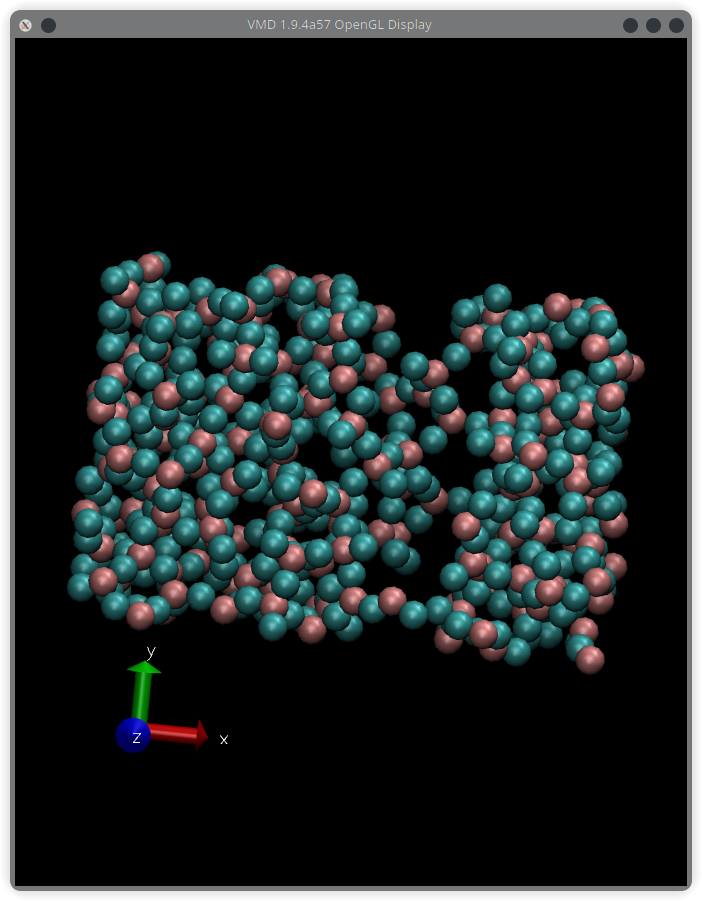
\includegraphics[scale=0.5]{Q3b_LF_Crack.png}\\
Water added in the crack:\\
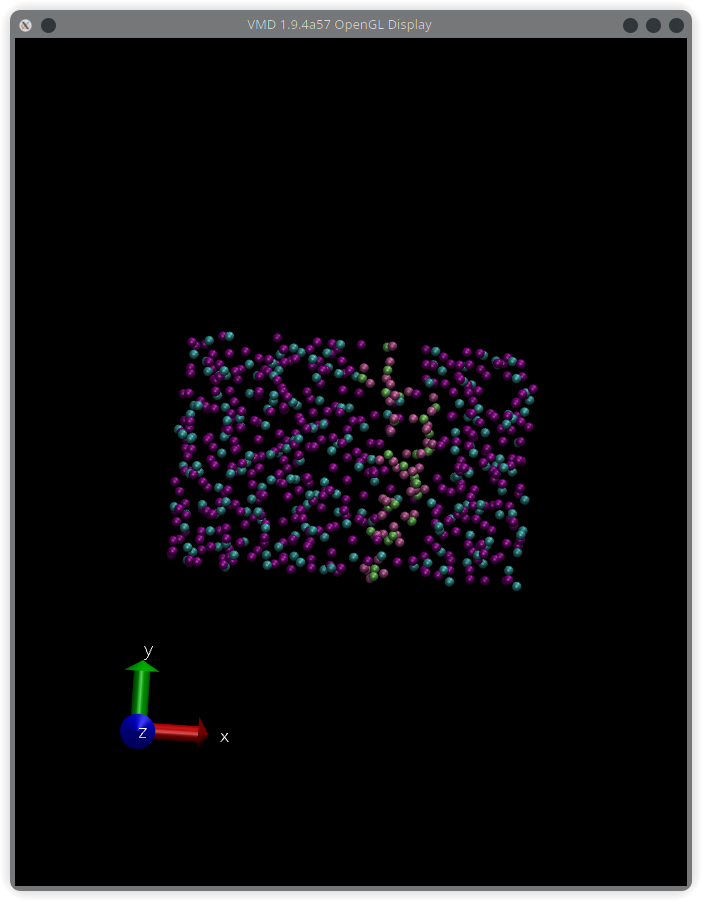
\includegraphics[scale=0.5]{Q3b_LF_Crackfill.png}\\
Energy variation with number of MC steps:\\
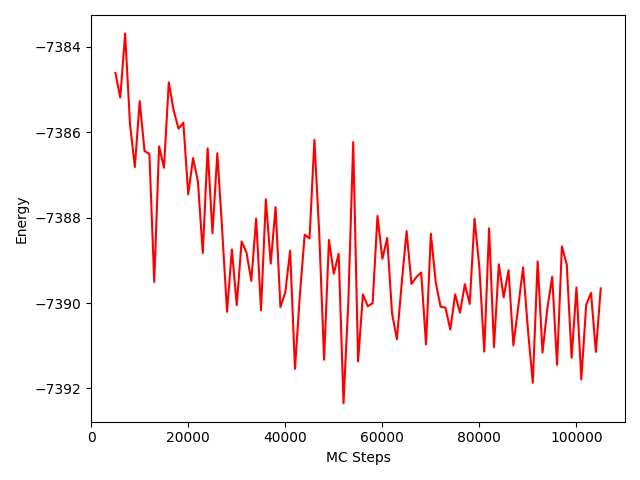
\includegraphics[scale=0.5]{Q3b_Crackfill_Energy_Plot.png}\\
As the number of MC steps increases, the energy shows a downward trend, as water molecules in the crack are filled, and the system tries to reach a state of lower energy.

\section{Question 4}
\subsection{A}
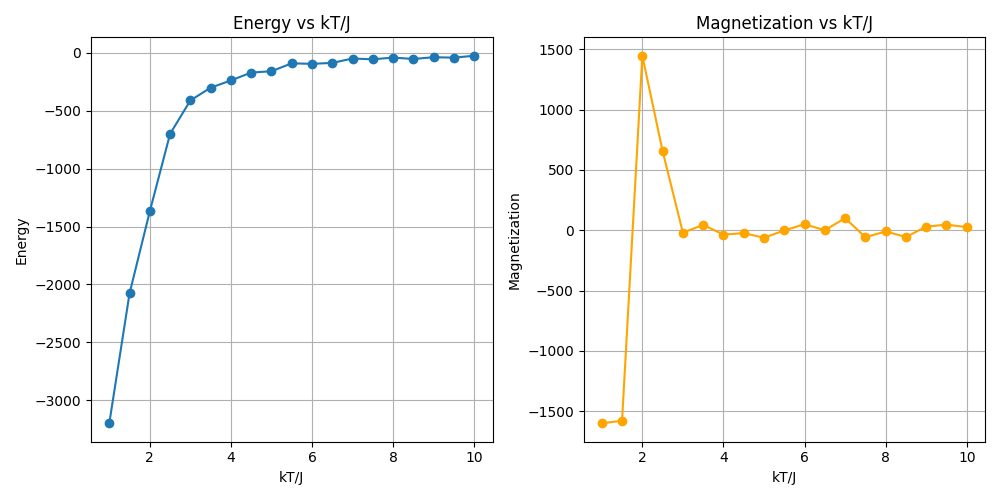
\includegraphics[scale=0.5]{Q4a_EMPlots.png}\\
The Material has a $T_C$ corresponding to 2.5. As the Temperature increases, the Material loses its internal magnetisation, and the spins start being random instead of aligned, leading to a net zero magnetisation.

At a paramagnetic state in absence of an external magnetic field, assuming $T>>T_C$, the spin visualisation is as follows:\\
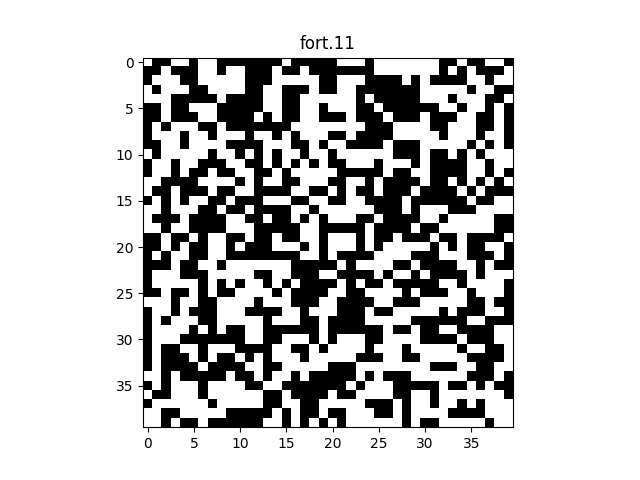
\includegraphics[scale=0.5]{fort.11.png}\\
At $T=T_C$, the spin visualisation is as follows:\\
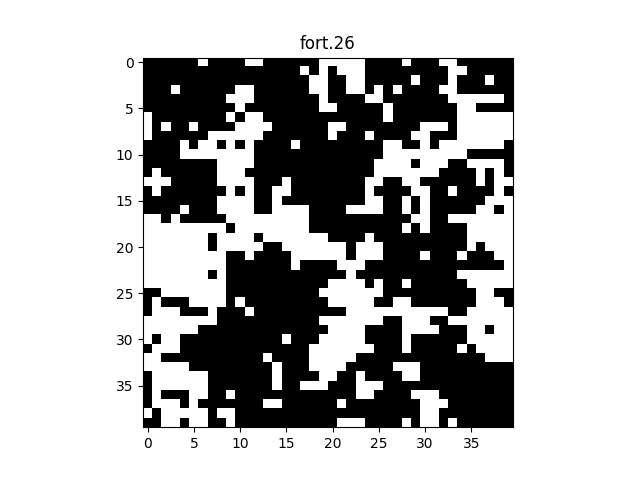
\includegraphics[scale=0.5]{fort.26.png}\\
The Material is ferromagnetic, when $T<<T_C$, where the spin visualisations are depicted as follows:\\
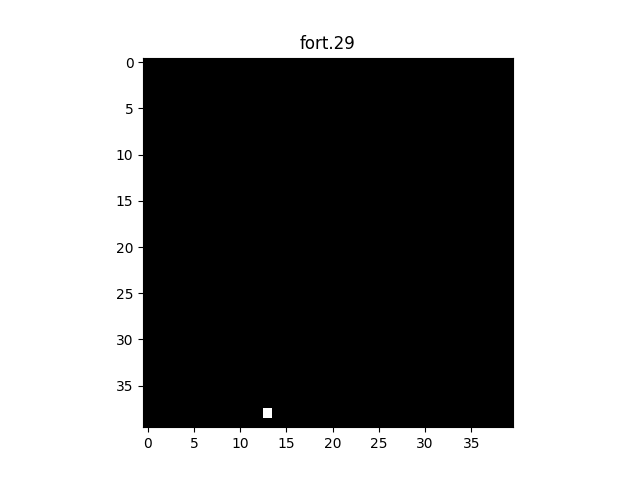
\includegraphics[scale=0.5]{fort.29.png}

\subsection{B}
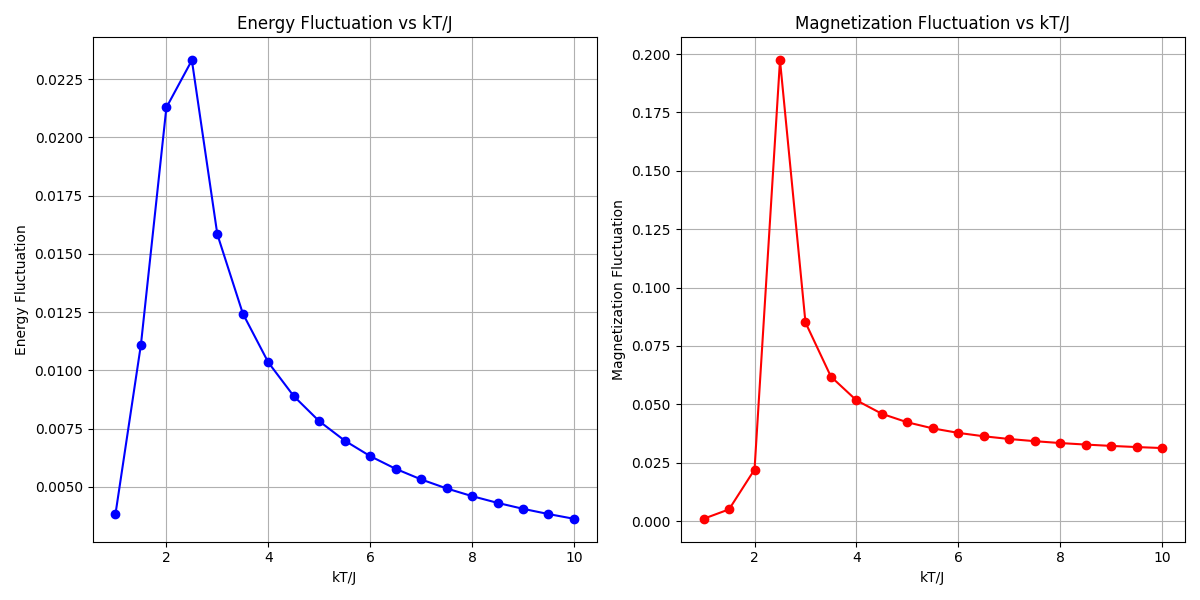
\includegraphics[scale=0.5]{Q4b_EMFluc.png}\\
Based on the plots, we can see that peak magnetic fluctuation occurs at $T_C$, before which there is little magnetic fluctuation, and after $T_C$ the magnetic fluctuations reduce. This can be correlated with the Ising model, where at ferromagnetic state, the spins are all of a single type, leading to low fluctuation. At $T_C$, Fluctuation is highest as the thermal energy leads to change in alignment of dipoles. When it is paramagnetic, there are no domains of magnetisation, and as such, fluctuation value is low.

\section{Question 5}
\subsection{A}
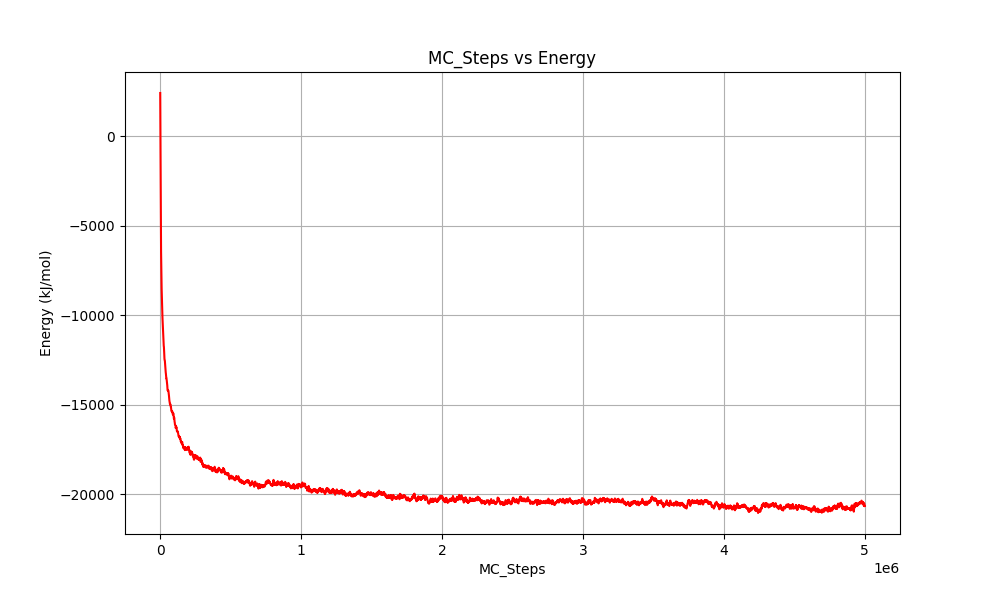
\includegraphics[scale=0.5]{Q5a.png}\\
With increasing number of Monte Carlo steps, the system reaches lower energy, and goes towards a more stable configuration. At the start of the simulation, the system is at an extremely high energy state, and the energy of the system quickly reduces as the simulation progresses and the number of MC steps increases. \\
\subsection{B}
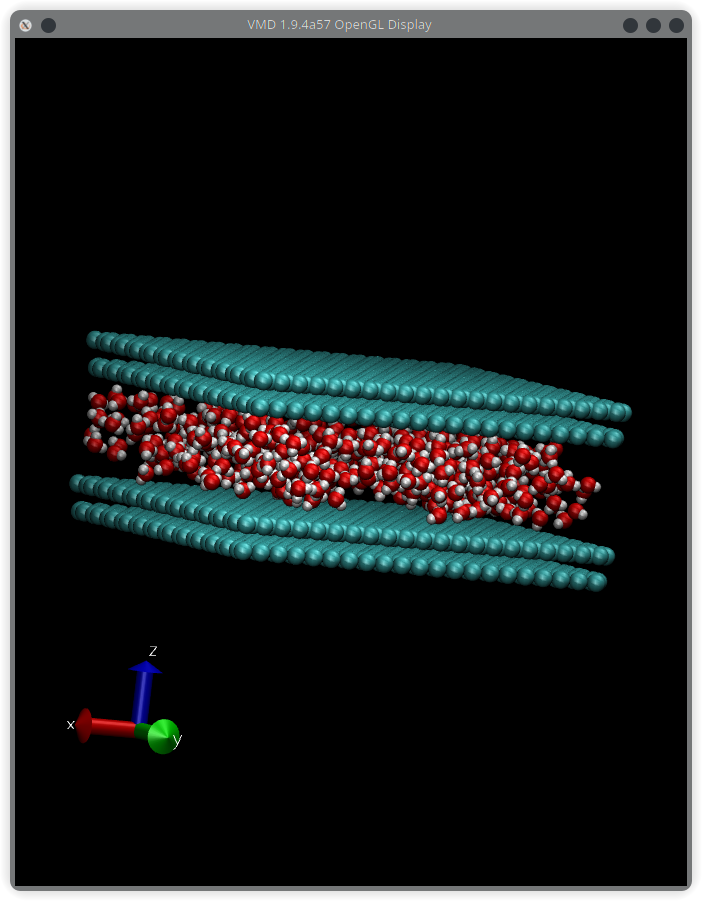
\includegraphics[scale=0.5]{Q5b.png}
\end{document}